% -----------------------------------------------------------------------------
\section{Recommended Best Practices}
\label{sec:bestpractices}
% -----------------------------------------------------------------------------
\twozeroone{\subsection{SBOL Namespaces}

Namespaces for different versions of SBOL SHOULD NOT be semantically mixed in the same document. For example, an SBOL 2.x \sbol{ComponentInstance} SHOULD NOT refer to an SBOL 1.x DNAComponent. However, namespaces for different versions MAY be present in the same document so long as they are semantically independent (that is, so long as objects belonging to these namespaces do not refer to each other). When multiple SBOL namespaces are present in a document, libraries SHOULD default to interpreting as SBOL only those objects belonging to the namespace for the most recent version of SBOL in the document. Any remaining objects belonging to any other SBOL namespace SHOULD be interpreted as \sbol{GenericTopLevel}s and custom \sbol{Annotation}s.}

\subsection{Use of the Version Property}

Once an SBOL object has been published where others might have access it (e.g., to an online repository), it might be the case that other objects come to depend on the particular contents of the published object. 
Thus, in order to avoid creating conflicting data, if a person wants to change the properties of a published object, they SHOULD do so by making a new copy of object that incorporates the change and has an \sbol{identity} property that contains a new \sbol{URI}.

The relationship between the old and new objects (i.e., that the new object was derived from the old object), however, is not visible unless it is explicitly declared.  This is RECOMMENDED to be done using the \sbol{persistentIdentity}, and \sbol{version} properties. The preferred practice for declaring such a relationship is to use the same \sbol{persistentIdentity} for both objects, but give the newer object a later \sbol{version}. Then, when the new object is published, it can be clear to both humans and machines that this object is intended to update the previously published object. In this way, when a user wants the latest version of an object, they can obtain it by referencing the object via its \sbol{persistentIdentity} and rely on a tool to find the object with that \sbol{persistentIdentity} and the latest \sbol{version}.

As stated in \ref{sec:version},  it is RECOMMENDED that version numbering follow
the conventions of semantic versions (\url{http://semver.org/}), particularly as implemented by Maven (\url{http://maven.apache.org/}).
This convention represents versions as sequences of numbers and qualifiers separated by the characters {\tt .} and {\tt -} and compared in lexicographical order (for example, 1 < 1.3.1 < 2.0-beta).  For a full explanation, see the linked resources.

\subsection{Compliant SBOL Objects}
\label{sec:compliant}

Maintaining unique \sbol{identity} \sbol{URI}s for all SBOL objects can be a very challenging implementation task.  To reduce this burden, users of SBOL 2.x are encouraged to follow a few simple rules when constructing the \sbol{identity} properties and related properties for SBOL objects.  When these rules are followed in constructing an SBOL object, we say that this object is \emph{compliant}. These rules are as follows:
\begin{enumerate}
\item The \sbol{identity} of a compliant SBOL object MUST begin with a \emph{URI prefix} that maps to a domain over which the user has control. Namely, the user can guarantee uniqueness of identities within this domain.
\item The \sbol{persistentIdentity} and \sbol{displayId} properties are REQUIRED of a compliant SBOL object.
\item The \sbol{persistentIdentity} of a compliant \sbol{TopLevel} object MUST end with a delimiter ('/', '\#', or ':') followed by the \sbol{displayId} of the object. 
\item The \sbol{persistentIdentity} of a compliant SBOL object that is not also a \sbol{TopLevel} object MUST begin with the \sbol{persistentIdentity} of its parent object and be immediately followed by a delimiter ('/', '\#', or ':') and the \sbol{displayId} of the compliant object.
\item If a compliant SBOL object is not given a \sbol{version}, then its \sbol{identity} and \sbol{persistentIdentity} properties MUST contain the same \sbol{URI}.
\item If a compliant SBOL object has a \sbol{version}, then its \sbol{identity} property MUST contain a \sbol{URI} of the form  "\refObj{persistentIdentity}/\refObj{version}".
\item The \sbol{version} of a compliant SBOL object that is not also a \sbol{TopLevel} object MUST contain the same \sbol{String} as the \sbol{version} property of the compliant object's parent object.
\item The \sbol{identity}, \sbol{persistentIdentity}, \sbol{displayId}, and \sbol{version} properties of a compliant SBOL object MUST NOT be changed once set.
\end{enumerate}

All examples in this specification use compliant \sbol{URI}s.

\subsection{Annotations: Embedded Objects vs. External References}

When annotating an SBOL document with additional information, there are
two general methods that can be used:
\begin{itemize}
\item Embed the information in the SBOL document, either as non-SBOL
  properties or \sbol{GenericTopLevel} objects.
\item Store the information separately and annotate the SBOL document
  with \sbol{URI}s that point to it.
\end{itemize}
In theory, either method can be used in any case. (Note that a third case not
discussed here is to use SBOL to annotate external objects with linking
to SBOL documents, rather than annotate SBOL documents with links external objects.)

In practice, 
embedding massive amounts of non-SBOL data into SBOL documents is likely
to cause problems for people and software tools trying to manage and
exchange such documents.  Therefore, it is RECOMMENDED that small amounts of information (e.g., design notes or preferred graphical layout) be embedded in the SBOL model, while large amounts of information (e.g., the contents of the scientific publication from which a model was derived or flow cytometry data that characterizes performance) be linked with URIs pointing to external resources.  The boundary between ``small'' and ``large'' is left deliberately vague, recognizing that it will likely depend on the particulars of a given SBOL application.

\subsection{Completeness and Validation}

RDF documents containing serialized SBOL objects might or might not be
entirely self-contained.  A SBOL document is self-contained or ``complete'' if every SBOL object referred to in the document is contained in the document.  It is RECOMMENDED that serializations be complete whenever practical.  In order words, when serializing an SBOL object, serialize all of the other objects that it points to, then serialize all of the other objects that these objects point to, etc., until the document is complete.

It is important to note that there is no guarantee that an RDF document
contains valid SBOL. When an RDF document is deserialized to SBOL
objects, the program doing so SHOULD verify that all of the property
values encoded therein have the right data type (e.g., that the object
pointed to by the \sbol{sequences} property of a
\sbol{ComponentDefinition} is really a \sbol{Sequence}).
For complete files, this validation can be carried out entirely locally. For files that are not complete, an implementation either needs to
have a means of validating those external references (e.g., by
retrieving them from various repositories), or it needs to mark them as
unverified and not depend on their correctness.

\subsection{Recommended Ontologies for External Terms}
\label{sec:recomm_ontologies}

External ontologies and controlled vocabularies are an integral part of SBOL. SBOL uses \sbol{URI}s to access existing biological information through these resources. New SBOL specific terms are defined only when necessary. For example, \sbol{ComponentDefinition} \sbolmult{types:CD}{types}, such as DNA or protein, are described using BioPAX terms. Similarly, the roles of a DNA \twozeroone{or RNA} \sbol{ComponentDefinition} are described via SO terms. Although RECOMMENDED ontologies have been indicated in relevant sections where possible, other resources providing similar terms can also be used. A summary of these external sources can be found in \ref{tbl:preferred_external_resources}.

\begin{table}[ht]
  \begin{edtable}{tabular}{p{3cm}p{1.5cm}p{4.5cm}p{6cm}}
    \toprule
    \textbf{SBOL Entity} & \textbf{Property} & \textbf{Preferred External Resource}
    & \textbf{More Information} \\
    \midrule
    \textbf{ComponentDefinition}  & types & BioPAX & \url{http://www.biopax.org}\\
                                  & types & SO (nucleic acid topology)& \url{http://www.sequenceontology.org}\\
    						   	  & roles & SO (\textit{DNA} or \textit{RNA}) & \url{http://www.sequenceontology.org}   \\
    						   	  & roles & CHEBI (\textit{small molecule}) & \url{https://www.ebi.ac.uk/chebi/}   \\
%    						   	  & roles & UniProt (if type is \textit{protein}??) \\   
    \textbf{Interaction}	      & types & SBO (occurring entity branch) & 
    \url{http://www.ebi.ac.uk/sbo/main/} \\
    \textbf{Participation}	      & roles & SBO (participant roles branch) &
    \url{http://www.ebi.ac.uk/sbo/main/} \\
    \textbf{Model}	      		  & language & EDAM & \url{http://bioportal.bioontology.org/ontologies/EDAM}     \\
    				      		  & framework & SBO (modeling framework branch) &
    \url{http://www.ebi.ac.uk/sbo/main/} \\
    \bottomrule
  \end{edtable}
  \caption{Preferred external resources from which to draw values for various SBOL properties.}
  \label{tbl:preferred_external_resources}
\end{table}

\twoonezero{The URIs for ontological terms SHOULD come from identifiers.org.  However, it is acceptable to use terms from purl.org as an alternative, for example when RDF tooling requires URIs to be represented as compliant QNames.  SBOL software may convert between these forms as required.}

\twozeroone{\subsection{Annotating Entities with Date \& Time}\label{sec:DateTime}
Entities in an SBOL document can be annotated with creation and modification date. It is RECOMMENDED that predicates, or properties, from DCMI Metadata Terms SHOULD be used to include date and time information. The \texttt{created} and \texttt{modified} terms SHOULD respectively be used to annotate SBOL entities with creation and modification dates. Date and time values SHOULD be expressed using the XML Schema \texttt{DateTime} datatype~\citep{Biron2004}. For example, "\texttt{2016-03-16T20:12:00Z}" specifies that the day is 16 March 2016 and the time is 20:12pm in UTC (Coordinated Universal Time). An example serialization is shown below:}

\lstsetsbol
\begin{lstlisting}
<?xml version="1.0" ?>
<rdf:RDF xmlns:pr="http://partsregistry.org" xmlns:rdf="http://www.w3.org/1999/02/22-rdf-syntax-ns#" xmlns:dcterms="http://purl.org/dc/terms/" xmlns:prov="http://www.w3.org/ns/prov#" xmlns:sbol="http://sbols.org/v2#">
  <sbol:CLASS_NAME rdf:about="...">
    <dcterms:created>DATE_TIME_STRING</dcterms:created>
    <dcterms:modified>DATE_TIME_STRING</dcterms:modified>
               ...
  </sbol:CLASS_NAME>
  ...
</rdf:RDF>
\end{lstlisting}

\twoonezero{\subsection{Adding Provenance}
\label{sec:provenance}
\label{sec:wasGeneratedBys}
Provenance is central to a range of quality control and attribution tasks within the Synthetic Biology design process. Tracking attribution and derivation of one resource from another is paramount for managing intellectual property purposes. Source designs are often modified in systematic ways to generate derived designs, for example, by applying codon optimization or systematically removing all of a class of restriction enzyme sites.  Documenting the transformation used, and any associated parameters, makes this explicit and potentially allows the process to be reproduced systematically. If a design has been used within other designs, and is later found to be defective, it is paramount that all uses of it, including uses of edited versions of the design, can be identified, and ideally replaced with a non-defective alternative. When importing data from external sources, it is important not only to attribute the original source (for example, GenBank), but also the tool used to perform the import, as this may have made arbitrary choices as to how to represent the source knowledge as SBOL. All these activities have in common that it is necessary to track what resource, and what transformation process was applied by whom to derive an SBOL design.

The PROV-O ontology (https://www.w3.org/TR/prov-o/) already defines a data model for provenance. PROV-O's \sbol{wasDerivedFroms} property was adopted in SBOL 2.x to describe the derivation of an SBOL entity from another in a light-weight provenance scheme.  Here, a subset of PROV-O is adopted for SBOL as a best practice to describe these activities in more detail\footnote{We thank Dr Paolo Missier from the School of Computing Science, Newcastle University for discussions regarding the use of PROV-O.}. PROV-O defines three core classes: \texttt{Entity}, \texttt{Activity} and \texttt{Agent}. An Agent (for example a software or a person) runs an Activity (according to a Plan) to generate one Entity from another. Although, PROV-O provides many other classes and rich set of terms. this specification describes the minimal subset of PROV-O that a provenance-aware SBOL tool should handle. This subset (\ref{uml:provenance}) includes the PROV-O's \sbol{Activity}, \sbol{Usage}, \sbol{Association}, \sbol{Agent} and \sbol{Plan} classes. Any SBOL's \sbol{Identified} object implicitly can act as an instance of PROV-O's \texttt{Entity} class and can include provenance through relationships to different activities. Resources representing \sbol{Agent}, \sbol{Activity} and \sbol{Plan} classes should be handled as \sbol{GenericTopLevel}, whilst \sbol{Usage} and \sbol{Association} resources should be nested within their parent activities. 

%Although the full-set of PROV-O terms can be used in SBOL documents, a subset of PROV-O is adopted as a best practice. It is advised that SBOL tools should at least understand this subset, defined in Figure \ref{uml:provenance}.  

Providers of provenance information are free to make use of more of PROV-O than is described here. It is acceptable for tools that understand more than this subset and use as much as they are able. Tools that only understand this subset must treat any additional data as annotations. Tools that are not aware of SBOL provenance at all must maintain and provide access to this information as annotations. This specification does not state what the newly added properties must point to. As long as they are resources that are consistent with the PROV-O property domains, they are legal. For example, a ComponentDefinition may be derived from another ComponentDefinition, but it would probably not make sense for it to be derived from a Collection.
}

\twotwozero{
The PROV-O specification permits that any kind of SBOL object may be used to generate another. The meaning of these relationships are specified using ontology terms for the \sbolmult{roles:U}{roles} properties on \sbol{Usage} and \sbol{Association} classes.  This specification gives users the flexibility to construct and track provenance histories for their own custom applications, but this flexibility also presents an obstacle to standardized data exchange. Therefore a simple ontology (see \ref{tbl:association_roles} and \ref{tbl:usage_roles}) has been adopted to describe common provenance connections expected in synthetic biology workflows, based on the design-build-test-learn formalization of engineering.

The design-build-test-learn cycle is a common theme in synthetic biology and engineering literature. The design-build-test-learn cycle is the scientific method applied to engineering. Stages of the cycle include designing an initial prototype, testing that prototype, analyzing its performance against specific metrics, learning what worked and what did not work, designing a new prototype based on what was learned, and completing the cycle again. Ideally each iteration of the cycle generates new understanding that feeds back into new cycles as alternative approaches or reformulated problems. Therefore, the design-build-test-learn cycle is a \textit{de facto} ontology upon which to base an SBOL data model for workflow abstraction. Other workflow activities in synthetic biology, such as analyzing, modeling, verifying, and evolving, by and large should fit into this design-build-test-learn abstraction. 

It is expected that users will develop their own ontology terms to specify how SBOL objects are used in a recipe, protocol, or computational analysis. However, these home-made ontologies will be very domain specific, and may not be intelligible to users working in another domain. For example a modeler should not be expected to understand an ontology of \sbol{Usage} \sbolmult{roles:U}{roles} for DNA assembly. The terms "design", "build", "test", and "learn" provide a high level workflow abstraction that allows tool-builders to quickly search for and isolate provenance histories relevant to their domain, while keeping track of the flow of data between different users working in different domains of synthetic biology. An example of how these terms are used is provided in \ref{images:design-build-test-learn}.

Provenance semantics defined through \sbol{wasGeneratedBys} relationships are distinctly different from versioning semantics. Generation of a new object is defined by the W3C PROV-O specification as follows:
\begin{quote}
...the completion of production of a new entity by an activity. This entity did not exist before generation and becomes available for usage after this generation.
\end{quote}
These semantics are somewhat different from the versioning semantics defined in section \ref{sec:version}. The SBOL specification defines a new version of an object as an update of a previously published object (and therefore a previously existing object). Therefore, an SBOL object which is "generated" from another SHOULD BE regarded as a new entity rather than a new version of an existing entity. However, this distinction is somewhat subjective (see Theseus paradox). Therefore, we RECOMMEND as a best practice that objects linked by Activities not be successive versions of each other, though this is left to the discretion of users and library developers.
} 

\twotwozero{
\begin{figure}[ht]
\begin{center}
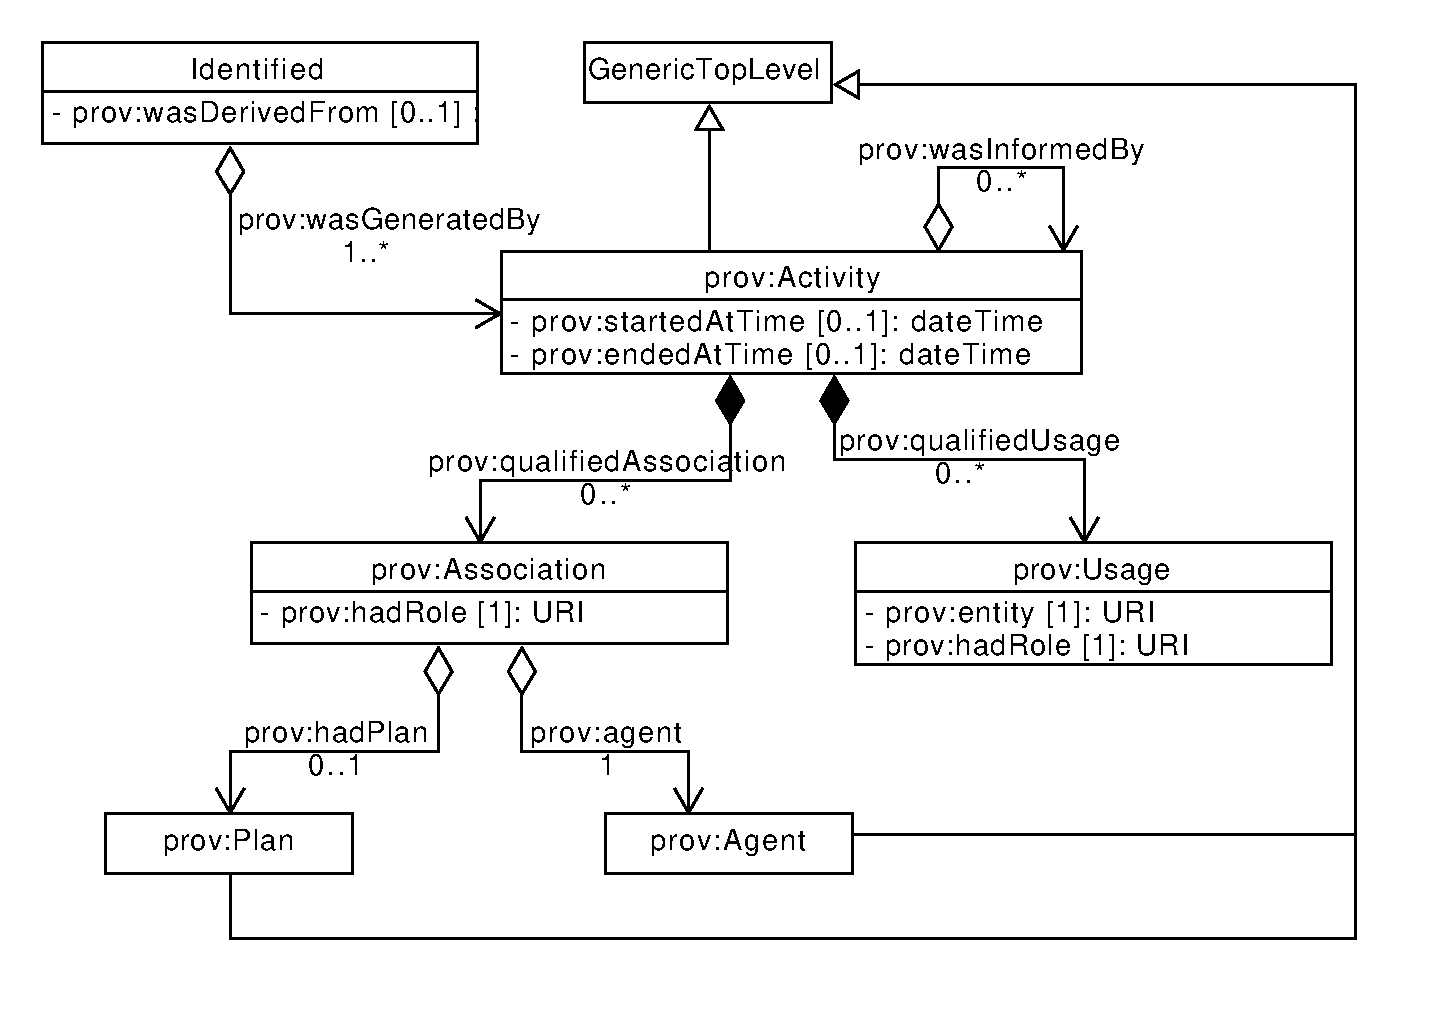
\includegraphics[scale=0.6]{uml/provenance}
\caption[]{Relationships between SBOL and PROV-O classes. The PROV-O classes \external{Activity}, \external{Plan}, and \external{Agent} are all serialized as \sbol{TopLevel} classes in an SBOL document.
\label{uml:provenance}}
\end{center}
\end{figure}
}

\twoonezero{
\subsubsection{Activity}
\label{sec:Activity}

A generated \texttt{Entity} is linked through a \texttt{wasGeneratedBy} relationship to an \sbol{Activity}, which is used to describe how different \sbol{Agent}s and other entities were used. An \sbol{Activity} is linked through a \sbol{associations} to \sbol{Association}s, to describe the role of agents, and is linked through \sbol{usages} to \sbol{Usage}s to describe the role of other entities used as part of the activity. Moreover, each \sbol{Activity} includes optional startedAtTime and endedAtTime properties. When using \sbol{Activity} to capture how an entity was derived, it is expected that any additional information needed will be attached as annotations. This may include software settings or textual notes. Activities can also be linked together using the \sbol{wasInformedBys} relationship to provide dependency without explicitly specifying start and end times.

\paragraph{The \sbolheading{associations} property}\label{sec:associations}
The \sbol{associations} property is OPTIONAL and MAY contain a set of \sbol{URI}s that refers to \sbol{Association} objects.

\paragraph{The \sbolheading{usages} property}\label{sec:usages}
The \sbol{usages} property is OPTIONAL and MAY contain a set of \sbol{URI}s that refers to \sbol{Usage} objects.

\paragraph{The \sbolheading{endedAtTime} property}\label{sec:endedAtTime}
The \sbol{endedAtTime} property is OPTIONAL and contains a DateTime (see section \ref{sec:DateTime}) value, indicating when the activity ended.

\paragraph{The \sbolheading{startedAtTime} property}\label{sec:startedAtTime}
The \sbol{startedAtTime} property is OPTIONAL and contains a DateTime (see section \ref{sec:DateTime}) value, indicating when the activity started.  If this property is present, then the \sbol{endedAtTime} property is REQUIRED.

\paragraph{The \sbolheading{wasInformedBys} property}\label{sec:wasInformedBys}
The \sbol{wasInformedBys} property is OPTIONAL and MAY contain a set of \sbol{URI}s that refers to other \sbol{Activity} objects.

\paragraph{Serialization}
The serialization of an \sbol{Activity} MUST have the following form:
%\twoonezero -end
}

\lstsetsbol
\begin{lstlisting}
<prov:Activity rdf:about="...">
  ... [\emph{properties inherited from identified}] ...
  [\emph{zero or more}]  <prov:qualifiedAssociation>
                   <prov:Association rdf:about="...">...</prov:Association>
                </prov:qualifiedAssociation> [\emph{elements}]
  [\emph{zero or more}]  <prov:qualifiedUsage>
                   <prov:Usage rdf:about="...">...</prov:Usage>
                </prov:qualifiedUsage> [\emph{elements}]             
  [\emph{zero or one}]  <prov:startedAtTime>...</prov:startedAtTime> [\emph{element}]
  [\emph{zero or one}]  <prov:endedAtTime>...</prov:startedAtTime> [\emph{element}] 
  [\emph{zero or more}]  <prov:wasInformedBy rdf:resource="..."/> [\emph{element}] 
</prov:Activity>
\end{lstlisting}

\twotwozero{
Note that the tags prov:qualifiedUsage and prov:qualifiedAssociation are used for \sbol{usages} and \sbol{associations}, respectively.
}

\twoonezero{
\subsubsection{Association}
\label{sec:Association}
An \sbol{Association} is linked to an \sbol{Agent} through the \sbol{agent} relationship. The \sbol{Association} includes the \sbolmult{roles:A}{roles} property to qualify the role of the \sbol{Agent} in the \sbol{Activity}.

\paragraph{The \sbolheading{agent} property}\label{sec:agent}
The \sbol{agent} property is REQUIRED and MUST contain a \sbol{URI} that refers to an \sbol{Agent} object.

\paragraph{The \sbolheading{roles} property}\label{sec:roles:A}
\twotwozero{ 
The \sbolmult{roles:A}{roles} property is an OPTIONAL set of \sbol{URI}s that refers to particular term(s) that describes the the role of the \sbol{agent} in the parent \sbol{Activity}. 
The recommended terms that are defined in \ref{tbl:association_roles} can be used to specify the kind of \sbol{Activity} performed by the \sbol{Agent}.
}
}

\twotwozero{
\begin{table}[H]
  \begin{edtable}{tabular}{lp{3.75in}}
    \toprule
    \textbf{URI for Association roles} & \textbf{Description} \\
    \midrule
    \url{http://sbols.org/v2\#design}	& Design describes the process by which a conceptual representation of an engineer's imagined and intended design for a biological system is derived, possibly from a predictive model or by modifying a pre-existing design. In the context of an \sbol{Association}, the term design indicates that the \sbol{agent} performed the parent {Activity} to generate a design\\
    \url{http://sbols.org/v2\#build}		& Build describes the process by which a biological construct, sample, or clone is implemented in the laboratory. In the context of an \sbol{Association}, the term build indicates that the \sbol{agent} performed the parent {Activity} to implement a design. More generally, the term may represent any kind of experimental manipulation of a biological sample, including propagating, passaging, or evolving cell lines.\\
    \url{http://sbols.org/v2\#test}		& Test describes the process of performing experimental measurements to characterize a synthetic biological construct. In the context of an \sbol{Association}, the \sbol{Agent} performed the parent {Activity} to perform experimental measurements resulting in raw data represented by \sbol{Attachment}s\\
    \url{http://sbols.org/v2\#learn}	&  Learn describes the process of analyzing experimental measurements to produce a new entity that represents biological knowledge. In the context of an \sbol{Association}, the \sbol{Agent} processed raw experimental data to produce an analysis. This process generates a new entity that represents biological knowledge, including tables or graphs contained by \sbol{Attachment}, a  \sbol{Model} produced by a fitting process, a consensus  \sbol{Sequence} derived from sequencing results, etc.\\
    \bottomrule
  \end{edtable}
  \caption{Terms to specify the \sbolmult{roles:A}{roles} property of an \sbol{Association}.}
  \label{tbl:association_roles}
\end{table}
} 

\twoonezero{
\paragraph{The \sbolheading{plan} property}\label{sec:plan}
The \sbol{plan} property is OPTIONAL and contains a URI that refers to a \sbol{Plan}.

\paragraph{Serialization}
The serialization of an \sbol{Association} MUST have the following form:

} 

\lstsetsbol
\begin{lstlisting}
<prov:Association rdf:about="...">
  ... [\emph{properties inherited from identified}] ...
  [\emph{zero or more}]  <prov:hadRole rdf:resource="..."/> [\emph{element}]
  [\emph{zero or one}]  <prov:hadPlan rdf:resource="..."/> [\emph{element}]
  [\emph{one}]  <prov:agent rdf:resource="..."/> [\emph{element}]
 </prov:Association>
\end{lstlisting}

\twotwozero{
Note that the tags prov:hadRole and prov:hadPlan are used for \sbolmult{roles:A}{roles} and \sbol{plan}, respectively.
}

\twoonezero{
\subsubsection{Usage}
\label{sec:Usage}
How different entities are used in an \sbol{Activity} is specified with the \sbol{Usage} class, which is linked from an \sbol{Activity} through the \sbol{Usage} relationship. A \sbol{Usage} is then linked to an \texttt{Entity} through the \texttt{Entity}'s URI and the role of this entity is qualified with the \sbolmult{roles:U}{roles} property. When the \sbol{wasDerivedFroms} property is used together with the full provenance described here, the entity pointed at by the \sbol{wasDerivedFroms} property MUST be included in a \sbol{Usage}.


\paragraph{The \sbolheading{entity} property}\label{sec:entity}
The \sbol{entity} property is REQUIRED and MUST contain a \sbol{URI} which MAY refer to an SBOL Identified object.

\paragraph{The \sbolheading{roles} property}\label{sec:roles:U}
\twotwozero{
The \sbolmult{roles:U}{roles} property is an OPTIONAL set of \sbol{URI}s that refer to particular term(s) describing the usage of an \sbol{entity} referenced by the \sbol{entity} property. Recommended terms that are defined in \ref{tbl:usage_roles} can be used to indicate how the referenced \sbol{entity} is being used in this \sbol{Activity}.
}
}

\twotwozero{
\begin{table}[H]
  \begin{edtable}{tabular}{lp{3.75in}}
    \toprule
    \textbf{URI for Usage roles} & \textbf{Description} \\
    \midrule
    \url{http://sbols.org/v2\#design}	& Design describes the process by which a conceptual representation of an engineer's imagined and intended design for a biological system is derived, possibly from a predictive model or by modifying a pre-existing design. In the context of a \sbol{Usage}, the term indicates that the referenced \sbol{entity} was generated by some previous design \sbol{Activity} and was used by the present \sbol{Activity} as a design for a new object.\\
    \url{http://sbols.org/v2\#build}		& Build describes the process by which a biological construct, sample, or clone is implemented in the laboratory. In the context of a \sbol{Usage}, the term  indicates that the referenced \sbol{entity} was generated by some previous build \sbol{Activity} and was used by the present \sbol{Activity} as a built object.\\
    \url{http://sbols.org/v2\#test}		& Test describes the process of performing experimental measurements to characterize a synthetic biological construct. In the context of a \sbol{Usage}, the term indicates that the referenced \sbol{entity} was generated by some previous test \sbol{Activity} and is used as test data in the present \sbol{Activity}.\\
    \url{http://sbols.org/v2\#learn}	&  Learn describes the process of analyzing experimental measurements to produce a new entity that represents biological knowledge. In the context of a \sbol{Usage}, the term indicates that the referenced \sbol{entity} was generated by some previous learn \sbol{Activity} and is used in the present \sbol{Activity} as a source of scientifically verified knowledge.\\
    \bottomrule
  \end{edtable}
  \caption{Terms to specify the \sbolmult{roles:U}{roles} property of a \sbol{Usage}.}
  \label{tbl:usage_roles}
\end{table}
} 

\twoonezero{
\paragraph{Serialization}
The serialization of an \sbol{Usage} MUST have the following form:
}

\lstsetsbol
\begin{lstlisting}
<prov:Usage rdf:about="...">
  ... [\emph{properties inherited from identified}] ...
  [\emph{zero or more}]  <prov:hadRole rdf:resource="..."/> [\emph{element}]
  [\emph{one}]  <prov:entity rdf:resource="..."/> [\emph{element}]
 </prov:Usage>
\end{lstlisting}

\twotwozero{
Note that the tag prov:hadPlan is used for \sbolmult{roles:U}{roles}.
}

\twoonezero{
\subsubsection{Plan}
\label{sec:Plan}
The Plan entity can be used as a place holder to describe the steps (for example scripts or lab protocols) taken when an \sbol{Agent} is used in a particular \sbol{Activity}. 

\paragraph{Serialization}
The serialization of an \sbol{Usage} MUST have the following form:

}%\twoonezero{ end

\lstsetsbol
\begin{lstlisting}
<prov:Plan rdf:about="...">
  ... [\emph{properties inherited from identified}] ...
  ... [\emph{other annotations}] ...
 </prov:Plan>
\end{lstlisting}

\twoonezero{
\subsubsection{Agent}
\label{sec:Agent}
Examples of agents are person, organization or software. These agents should be annotated with additional information, such as software version, needed to be able to run the same software again.

\paragraph{Serialization}
The serialization of an \sbol{Agent} MUST have the following form:

}%\twoonezero{ end

\lstsetsbol
\begin{lstlisting}
<prov:Agent rdf:about="...">
  ... [\emph{properties inherited from identified}] ...
  ... [\emph{other annotations}] ...
 </prov:Agent>
\end{lstlisting}


\twoonezero{
\paragraph{Example - Codon optimization}
Codon optimization is a practical real-wold example where provenance properties can be applied. Using the current specification, the relationship between an original CDS and the codon-optimized version could simply be represented using the prov:wasDerivedFrom predicate, in a light-weight form. With more comprehensive use of the PROV ontology, the codon optimization can be represented as an \sbol{Activity}. This \sbol{Activity} can then include additional information, such as the \sbol{Agent} responsible (in this case, codon-optimizing software), and additional parameters.

}%\twoonezero{ end

\lstsetsbol
\begin{lstlisting}
<?xml version="1.0" ?>
<rdf:RDF xmlns:prov="http://www.w3.org/ns/prov#" xmlns:rdf="http://www.w3.org/1999/02/22-rdf-syntax-ns#" xmlns:myapp="http://myapp.com/" xmlns:sbol="http://sbols.org/v2#" xmlns:dcterms="http://purl.org/dc/terms/">
  <sbol:ComponentDefinition rdf:about="http://myapp.com/codon_optimized">
    <sbol:persistentIdentity rdf:resource="http://myapp.com/codon_optimized"/>
    <sbol:displayId>codon_optimized</sbol:displayId>
    <prov:wasDerivedFrom rdf:resource="http://myapp.com/non_codon_optimized"/>
    <prov:wasGeneratedBy rdf:resource="http://myapp.com/codon_optimization_activity"/>
    <dcterms:title>Codon optimized CDS</dcterms:title>
    <sbol:type rdf:resource="http://www.biopax.org/release/biopax-level3.owl#DnaRegion"/>
    <sbol:role rdf:resource="http://identifiers.org/so/SO:0000316"/>
  </sbol:ComponentDefinition>
  <sbol:ComponentDefinition rdf:about="http://myapp.com/non_codon_optimized">
    <sbol:persistentIdentity rdf:resource="http://myapp.com/non_codon_optimized"/>
    <sbol:displayId>non_codon_optimized</sbol:displayId>
    <dcterms:title>Non Codon optimized CDS</dcterms:title>
    <sbol:type rdf:resource="http://www.biopax.org/release/biopax-level3.owl#DnaRegion"/>
    <sbol:role rdf:resource="http://identifiers.org/so/SO:0000316"/>
  </sbol:ComponentDefinition>
  <prov:Activity rdf:about="http://myapp.com/codon_optimization_activity">
    <sbol:persistentIdentity rdf:resource="http://myapp.com/codon_optimization_activity"/>
    <sbol:displayId>codon_optimization_activity</sbol:displayId>
    <dcterms:title>Codon Optimization Activity</dcterms:title>
    <prov:qualifiedAssociation>
      <prov:Association rdf:about="http://myapp.com/codon_optimization_activity/association">
        <sbol:persistentIdentity rdf:resource="http://myapp.com/codon_optimization_activity/association"/>
        <sbol:displayId>association</sbol:displayId>
        <prov:hadRole rdf:resource="http://myapp.com/codonoptimizer"/>
        <prov:agent rdf:resource="http://myapp.com/codon_optimization_software"/>
      </prov:Association>
    </prov:qualifiedAssociation>
    <prov:qualifiedUsage>
      <prov:Usage rdf:about="http://myapp.com/codon_optimization_activity/usage">
        <sbol:persistentIdentity rdf:resource="http://myapp.com/codon_optimization_activity/usage"/>
        <sbol:displayId>usage</sbol:displayId>
        <prov:hadRole rdf:resource="http://sbols.org/v2#source"/>
        <prov:entity rdf:resource="http://myapp.com/non_codon_optimized"/>
      </prov:Usage>
    </prov:qualifiedUsage>
  </prov:Activity>
  <prov:Agent rdf:about="http://myapp.com/codon_optimization_software">
    <sbol:persistentIdentity rdf:resource="http://myapp.com/codon_optimization_software"/>
    <sbol:displayId>codon_optimization_software</sbol:displayId>
    <dcterms:title>Codon Optimization Software</dcterms:title>
  </prov:Agent>
</rdf:RDF>
\end{lstlisting}

\twoonezero{
\paragraph{Example - Deriving strains}
Bacterial strains are often derived from other strains through modifications such as gene knockouts or mutations. For example, the \texttt{Bacillus subtilis} 168 strain was derived from the NCIMB3610 strain in the 1940s through x-radiation. \textit{B. subtilis} 168 is a laboratory strain and has several advantages as a model organism in synthetic biology. Particularly, the 168 strain is easy to transform and is not motile, facilitating the analysis of engineered cells. The parent strain, on the other hand, is motile but more difficult to transform. The example below shows the derivation of the 168 strain using the new provenance classes.

}%twoonezero end

\lstsetsbol
\begin{lstlisting}
<?xml version="1.0" ?>
<rdf:RDF xmlns:prov="http://www.w3.org/ns/prov#" xmlns:rdf="http://www.w3.org/1999/02/22-rdf-syntax-ns#" xmlns:myapp="http://myapp.com/" xmlns:sbol="http://sbols.org/v2#" xmlns:dcterms="http://purl.org/dc/terms/">
  <sbol:ComponentDefinition rdf:about="http://myapp.com/bsubtilisncimb3610">
    <sbol:persistentIdentity rdf:resource="http://myapp.com/bsubtilisncimb3610"/>
    <sbol:displayId>bsubtilisncimb3610</sbol:displayId>
    <dcterms:title>Bacillus subtilis NCIMB3610</dcterms:title>
    <sbol:type rdf:resource="http://www.biopax.org/release/biopax-level3.owl#DnaRegion"/>
    <sbol:role rdf:resource="http://identifiers.org/so/SO:0000316"/>
  </sbol:ComponentDefinition>
  <sbol:ComponentDefinition rdf:about="http://myapp.com/bsubtilis168">
    <sbol:persistentIdentity rdf:resource="http://myapp.com/bsubtilis168"/>
    <sbol:displayId>bsubtilis168</sbol:displayId>
    <prov:wasDerivedFrom rdf:resource="http://myapp.com/bsubtilisncimb3610"/>
    <prov:wasGeneratedBy rdf:resource="http://myapp.com/xraymutagenesis"/>
    <dcterms:title>Bacillus subtilis 168</dcterms:title>
    <sbol:type rdf:resource="http://www.biopax.org/release/biopax-level3.owl#DnaRegion"/>
    <sbol:role rdf:resource="http://identifiers.org/so/SO:0000316"/>
  </sbol:ComponentDefinition>
  <prov:Activity rdf:about="http://myapp.com/xraymutagenesis">
    <sbol:persistentIdentity rdf:resource="http://myapp.com/xraymutagenesis"/>
    <sbol:displayId>xraymutagenesis</sbol:displayId>
    <dcterms:title>X-ray mutagenesis</dcterms:title>
    <prov:qualifiedAssociation>
      <prov:Association rdf:about="http://myapp.com/xraymutagenesis/association">
        <sbol:persistentIdentity rdf:resource="http://myapp.com/xraymutagenesis/association"/>
        <sbol:displayId>association</sbol:displayId>
        <prov:hadRole rdf:resource="http://myapp.com/mutagen"/>
        <prov:agent rdf:resource="http://myapp.com/x_ray"/>
      </prov:Association>
    </prov:qualifiedAssociation>
    <prov:qualifiedUsage>
      <prov:Usage rdf:about="http://myapp.com/xraymutagenesis/usage">
        <sbol:persistentIdentity rdf:resource="http://myapp.com/xraymutagenesis/usage"/>
        <sbol:displayId>usage</sbol:displayId>
        <prov:hadRole rdf:resource="http://sbols.org/v2#source"/>
        <prov:entity rdf:resource="http://myapp.com/bsubtilisncimb3610"/>
      </prov:Usage>
    </prov:qualifiedUsage>
  </prov:Activity>
  <prov:Agent rdf:about="http://myapp.com/x_ray">
    <sbol:persistentIdentity rdf:resource="http://myapp.com/x_ray"/>
    <sbol:displayId>x_ray</sbol:displayId>
    <dcterms:title>X-ray</dcterms:title>
  </prov:Agent>
</rdf:RDF>
\end{lstlisting}

\twotwozero{
\paragraph{Example - Design-build-test-learn Workflow}
This particular example represents an idealized workflow for model-based design. The workflow begins with a Model which describes the hypothesized behavior of a biological device. Using a computational tool, a new Design (ModuleDefinition) is composed of biological parts which links back to its Model. A genetic construct is then produced in the laboratory via an assembly protocol, and this biological sample is represented by a Build (Implementation). Once constructed, the Build is then characterized in the laboratory using an automated measurement protocol on a Tecan plate reader, thus generating Test data (represented by an Attachment). Finally, a new Model is derived from these data using some a fitting algorithm implemented in the Python programming language. The final Model may not match the beginning Model, as the observed behavior may not match the prediction. This example illustrates one complete iteration through a design-build-test-learn cycle, as shown in  \ref{images:design-build-test-learn}.
}%twotwozero end

\begin{figure}[ht]
\begin{center}
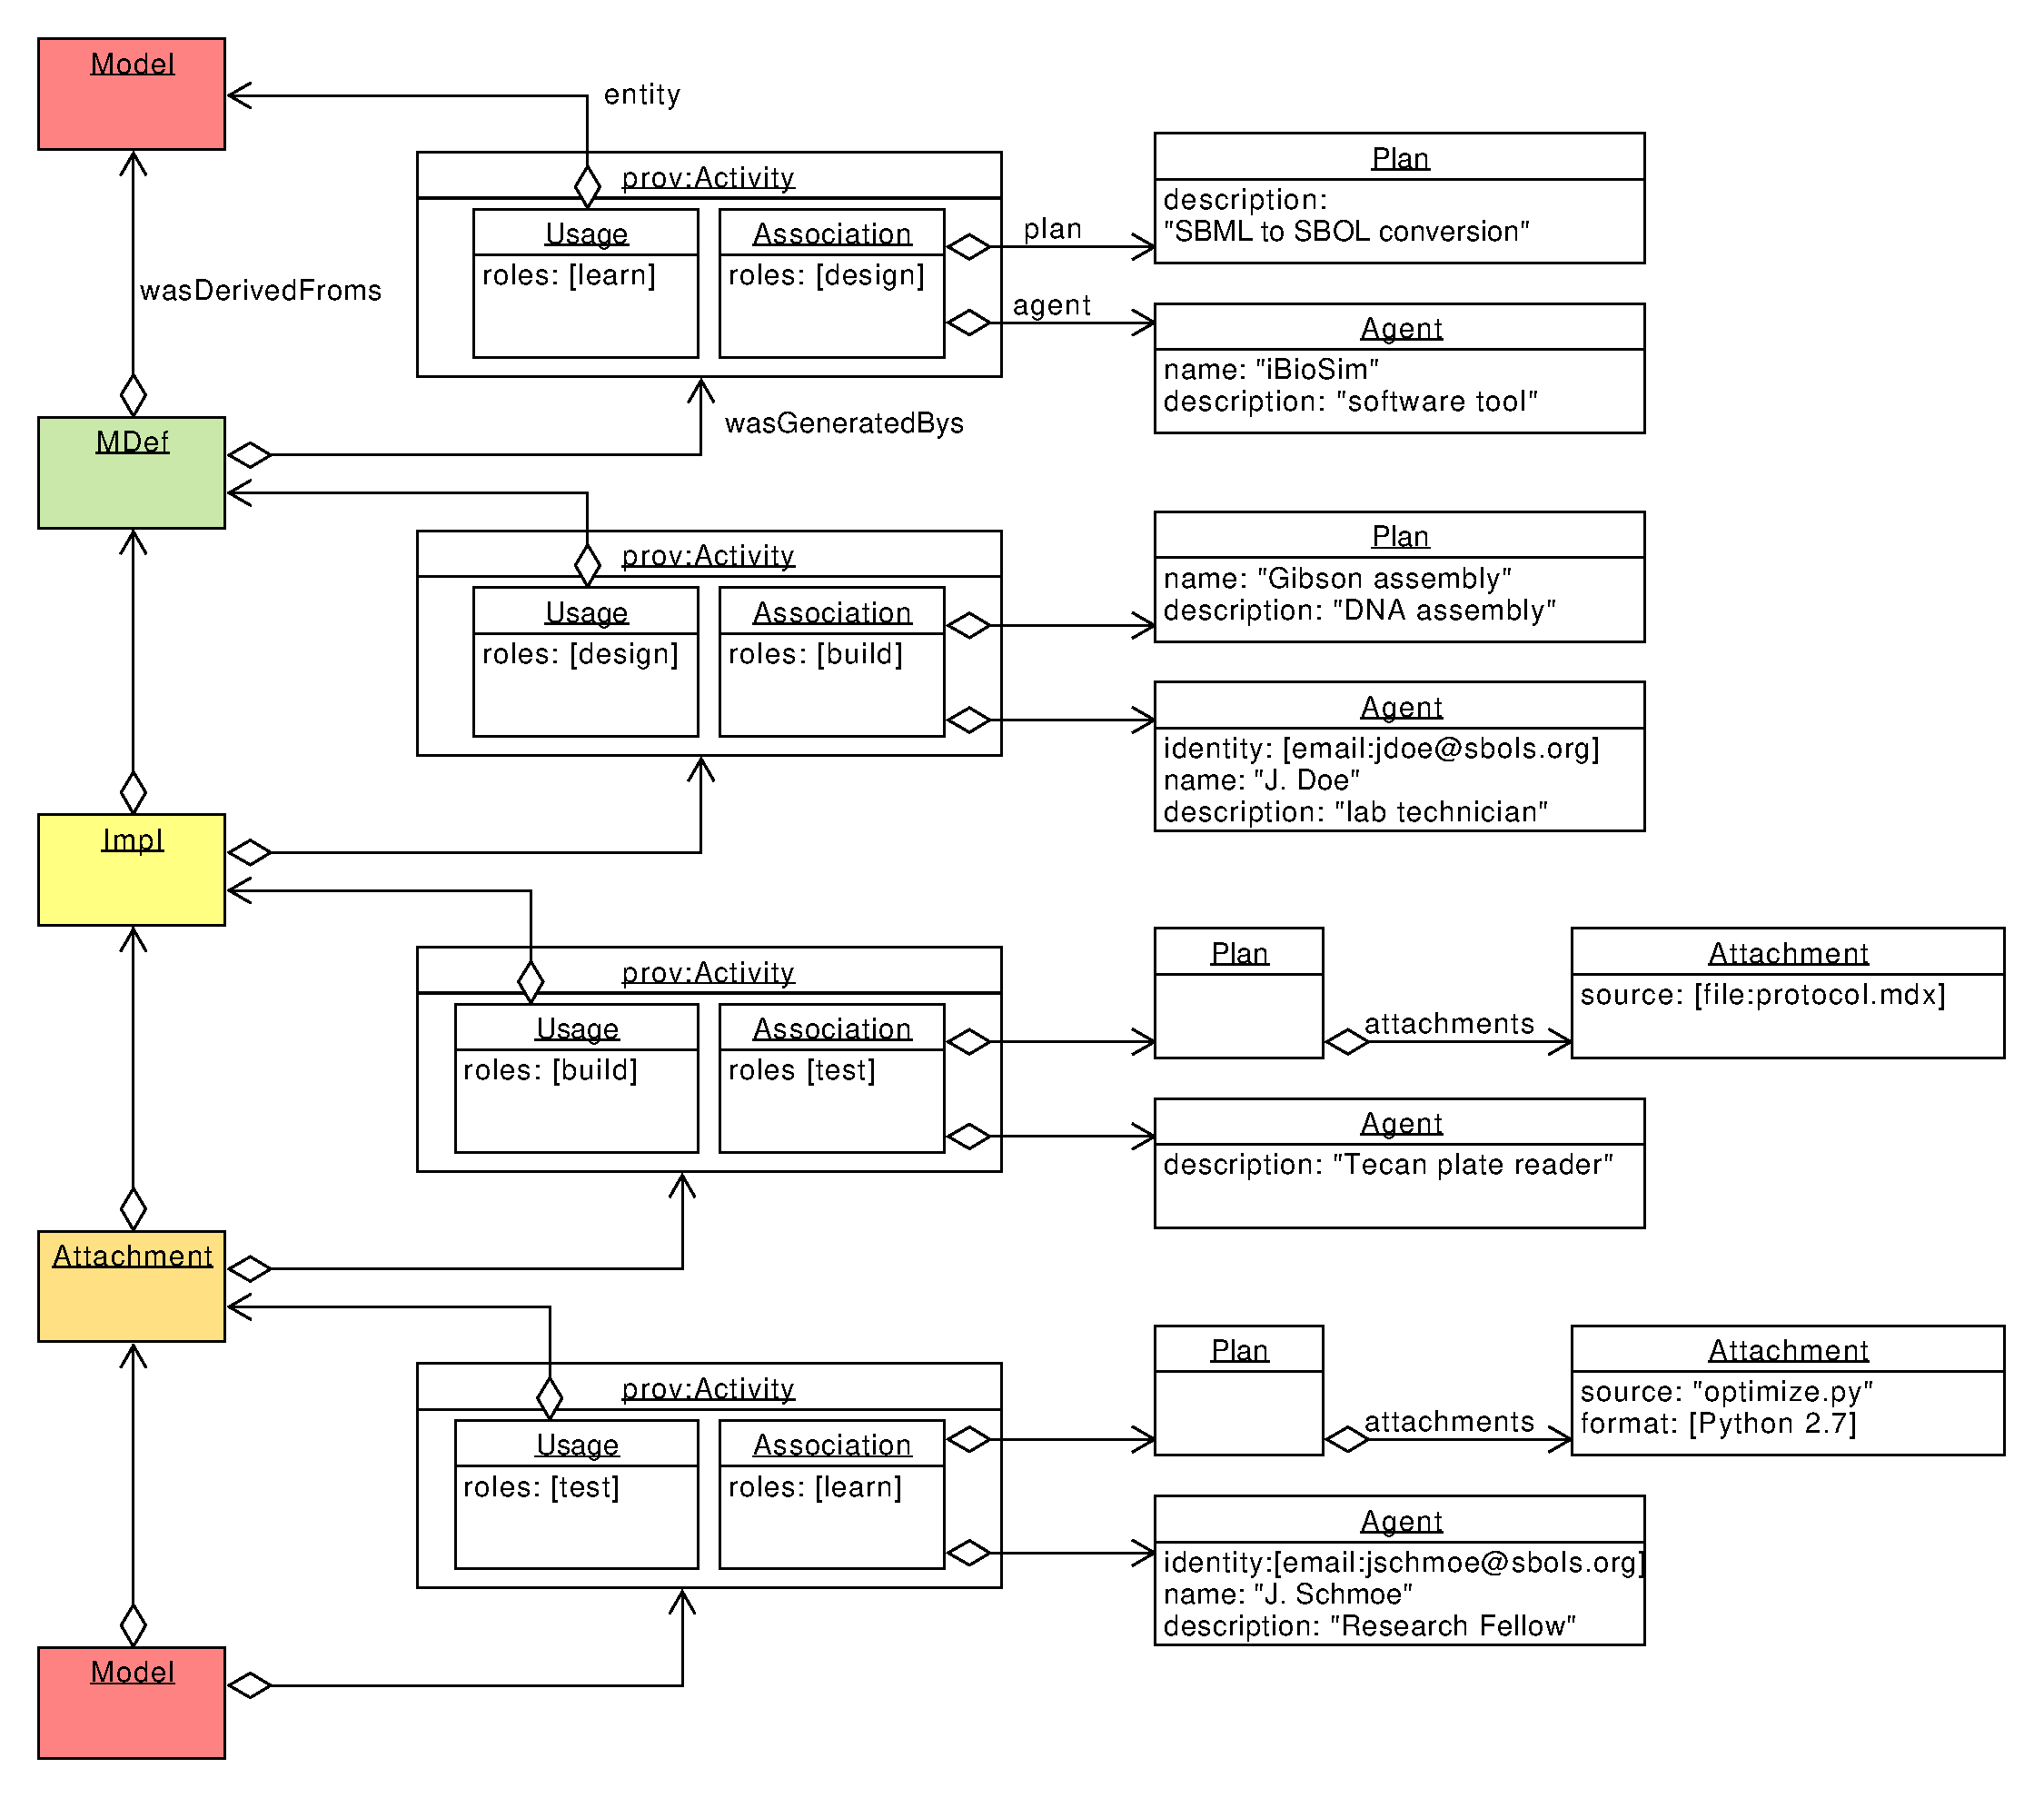
\includegraphics[width=\linewidth]{images/design-build-test-learn}
\caption[]{An example data structure representing an idealized workflow for model-based
design}
\label{images:design-build-test-learn}
\end{center}
\end{figure}

\lstsetsbol
\begin{lstlisting}
<?xml version="1.0" encoding="utf-8"?>
<rdf:RDF xmlns:dcterms="http://purl.org/dc/terms/"
   xmlns:prov="http://www.w3.org/ns/prov#"
   xmlns:rdf="http://www.w3.org/1999/02/22-rdf-syntax-ns#"
   xmlns:sbol="http://sbols.org/v2#">
  <prov:Activity rdf:about="http://examples.org/Activity/generate_build/1.0.0">
    <sbol:displayId>generate_build</sbol:displayId>
    <sbol:persistentIdentity rdf:resource="http://examples.org/Activity/generate_build"/>
    <sbol:version>1.0.0</sbol:version>
    <prov:qualifiedUsage>
      <prov:Usage rdf:about="http://examples.org/Activity/generate_build/design_usage/1.0.0">
        <sbol:displayId>design_usage</sbol:displayId>
        <sbol:persistentIdentity rdf:resource="http://examples.org/Activity/generate_build/design_usage"/>
        <sbol:version>1.0.0</sbol:version>
        <prov:entity rdf:resource="http://examples.org/ModuleDefinition/design/1.0.0"/>
        <prov:hadRole rdf:resource="http://sbols.org/v2#design"/>
      </prov:Usage>
    </prov:qualifiedUsage>
    <prov:qualifiedUsage>
      <prov:Usage rdf:about="http://examples.org/Activity/generate_build/usage/1.0.0">
        <sbol:displayId>usage</sbol:displayId>
        <sbol:persistentIdentity rdf:resource="http://examples.org/Activity/generate_build/usage"/>
        <sbol:version>1.0.0</sbol:version>
      </prov:Usage>
    </prov:qualifiedUsage>
    <prov:qualifiedAssociation>
      <prov:Association rdf:about="http://examples.org/Activity/generate_build/association/1.0.0">
        <sbol:displayId>association</sbol:displayId>
        <sbol:persistentIdentity rdf:resource="http://examples.org/Activity/generate_build/association"/>
        <sbol:version>1.0.0</sbol:version>
        <prov:hadRole rdf:resource="http://sbols.org/v2#build"/>
      </prov:Association>
    </prov:qualifiedAssociation>
  </prov:Activity>
  <prov:Activity rdf:about="http://examples.org/Activity/generate_design/1.0.0">
    <sbol:displayId>generate_design</sbol:displayId>
    <sbol:persistentIdentity rdf:resource="http://examples.org/Activity/generate_design"/>
    <sbol:version>1.0.0</sbol:version>
    <prov:qualifiedUsage>
      <prov:Usage rdf:about="http://examples.org/Activity/generate_design/predicted_usage/1.0.0">
        <sbol:displayId>predicted_usage</sbol:displayId>
        <sbol:persistentIdentity rdf:resource="http://examples.org/Activity/generate_design/predicted_usage"/>
        <sbol:version>1.0.0</sbol:version>
        <prov:entity rdf:resource="http://examples.org/Model/predicted/1.0.0"/>
        <prov:hadRole rdf:resource="http://sbols.org/v2#learn"/>
      </prov:Usage>
    </prov:qualifiedUsage>
    <prov:qualifiedUsage>
      <prov:Usage rdf:about="http://examples.org/Activity/generate_design/usage/1.0.0">
        <sbol:displayId>usage</sbol:displayId>
        <sbol:persistentIdentity rdf:resource="http://examples.org/Activity/generate_design/usage"/>
        <sbol:version>1.0.0</sbol:version>
      </prov:Usage>
    </prov:qualifiedUsage>
    <prov:qualifiedAssociation>
      <prov:Association rdf:about="http://examples.org/Activity/generate_design/association/1.0.0">
        <sbol:displayId>association</sbol:displayId>
        <sbol:persistentIdentity rdf:resource="http://examples.org/Activity/generate_design/association"/>
        <sbol:version>1.0.0</sbol:version>
        <prov:hadRole rdf:resource="http://sbols.org/v2#design"/>
      </prov:Association>
    </prov:qualifiedAssociation>
  </prov:Activity>
  <prov:Activity rdf:about="http://examples.org/Activity/generate_observed/1.0.0">
    <sbol:displayId>generate_observed</sbol:displayId>
    <sbol:persistentIdentity rdf:resource="http://examples.org/Activity/generate_observed"/>
    <sbol:version>1.0.0</sbol:version>
    <prov:qualifiedUsage>
      <prov:Usage rdf:about="http://examples.org/Activity/generate_observed/test_data_usage/1.0.0">
        <sbol:displayId>test_data_usage</sbol:displayId>
        <sbol:persistentIdentity rdf:resource="http://examples.org/Activity/generate_observed/test_data_usage"/>
        <sbol:version>1.0.0</sbol:version>
        <prov:entity rdf:resource="http://examples.org/Attachment/test_data/1.0.0"/>
        <prov:hadRole rdf:resource="http://sbols.org/v2#test"/>
      </prov:Usage>
    </prov:qualifiedUsage>
    <prov:qualifiedUsage>
      <prov:Usage rdf:about="http://examples.org/Activity/generate_observed/usage/1.0.0">
        <sbol:displayId>usage</sbol:displayId>
        <sbol:persistentIdentity rdf:resource="http://examples.org/Activity/generate_observed/usage"/>
        <sbol:version>1.0.0</sbol:version>
      </prov:Usage>
    </prov:qualifiedUsage>
    <prov:qualifiedAssociation>
      <prov:Association rdf:about="http://examples.org/Activity/generate_observed/association/1.0.0">
        <sbol:displayId>association</sbol:displayId>
        <sbol:persistentIdentity rdf:resource="http://examples.org/Activity/generate_observed/association"/>
        <sbol:version>1.0.0</sbol:version>
        <prov:hadRole rdf:resource="http://sbols.org/v2#learn"/>
      </prov:Association>
    </prov:qualifiedAssociation>
  </prov:Activity>
  <prov:Activity rdf:about="http://examples.org/Activity/generate_test_data/1.0.0">
    <sbol:displayId>generate_test_data</sbol:displayId>
    <sbol:persistentIdentity rdf:resource="http://examples.org/Activity/generate_test_data"/>
    <sbol:version>1.0.0</sbol:version>
    <prov:qualifiedUsage>
      <prov:Usage rdf:about="http://examples.org/Activity/generate_test_data/build_usage/1.0.0">
        <sbol:displayId>build_usage</sbol:displayId>
        <sbol:persistentIdentity rdf:resource="http://examples.org/Activity/generate_test_data/build_usage"/>
        <sbol:version>1.0.0</sbol:version>
        <prov:entity rdf:resource="http://examples.org/Implementation/build/1.0.0"/>
        <prov:hadRole rdf:resource="http://sbols.org/v2#build"/>
      </prov:Usage>
    </prov:qualifiedUsage>
    <prov:qualifiedUsage>
      <prov:Usage rdf:about="http://examples.org/Activity/generate_test_data/usage/1.0.0">
        <sbol:displayId>usage</sbol:displayId>
        <sbol:persistentIdentity rdf:resource="http://examples.org/Activity/generate_test_data/usage"/>
        <sbol:version>1.0.0</sbol:version>
      </prov:Usage>
    </prov:qualifiedUsage>
    <prov:qualifiedAssociation>
      <prov:Association rdf:about="http://examples.org/Activity/generate_test_data/association/1.0.0">
        <sbol:displayId>association</sbol:displayId>
        <sbol:persistentIdentity rdf:resource="http://examples.org/Activity/generate_test_data/association"/>
        <sbol:version>1.0.0</sbol:version>
        <prov:hadRole rdf:resource="http://sbols.org/v2#test"/>
      </prov:Association>
    </prov:qualifiedAssociation>
  </prov:Activity>
  <sbol:Attachment rdf:about="http://examples.org/Attachment/test_data/1.0.0">
    <sbol:displayId>test_data</sbol:displayId>
    <sbol:persistentIdentity rdf:resource="http://examples.org/Attachment/test_data"/>
    <sbol:size>0</sbol:size>
    <sbol:version>1.0.0</sbol:version>
    <prov:wasGeneratedBy rdf:resource="http://examples.org/Activity/generate_observed/1.0.0"/>
  </sbol:Attachment>
  <sbol:Implementation rdf:about="http://examples.org/Implementation/build/1.0.0">
    <sbol:displayId>build</sbol:displayId>
    <sbol:persistentIdentity rdf:resource="http://examples.org/Implementation/build"/>
    <sbol:version>1.0.0</sbol:version>
    <prov:wasGeneratedBy rdf:resource="http://examples.org/Activity/generate_test_data/1.0.0"/>
  </sbol:Implementation>
  <sbol:Model rdf:about="http://examples.org/Model/observed/1.0.0">
    <sbol:displayId>observed</sbol:displayId>
    <sbol:framework rdf:resource="http://identifiers.org/biomodels.sbo/SBO:0000062"/>
    <sbol:language rdf:resource="http://identifiers.org/edam/format_2585"/>
    <sbol:persistentIdentity rdf:resource="http://examples.org/Model/observed"/>
    <sbol:version>1.0.0</sbol:version>
  </sbol:Model>
  <sbol:Model rdf:about="http://examples.org/Model/predicted/1.0.0">
    <sbol:displayId>predicted</sbol:displayId>
    <sbol:framework rdf:resource="http://identifiers.org/biomodels.sbo/SBO:0000062"/>
    <sbol:language rdf:resource="http://identifiers.org/edam/format_2585"/>
    <sbol:persistentIdentity rdf:resource="http://examples.org/Model/predicted"/>
    <sbol:version>1.0.0</sbol:version>
    <prov:wasGeneratedBy rdf:resource="http://examples.org/Activity/generate_design/1.0.0"/>
  </sbol:Model>
  <sbol:ModuleDefinition rdf:about="http://examples.org/ModuleDefinition/design/1.0.0">
    <sbol:displayId>design</sbol:displayId>
    <sbol:persistentIdentity rdf:resource="http://examples.org/ModuleDefinition/design"/>
    <sbol:version>1.0.0</sbol:version>
    <prov:wasGeneratedBy rdf:resource="http://examples.org/Activity/generate_build/1.0.0"/>
  </sbol:ModuleDefinition>
</rdf:RDF>
\end{lstlisting}


